%% -*- coding:utf-8 -*-
\begin{figure}
\centering
\ifpdf
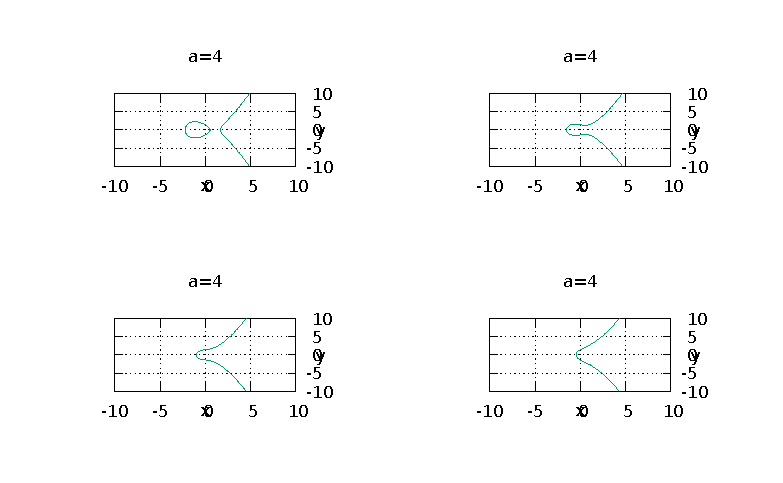
\includegraphics[angle=0]
{./add/discretmath/picelliptic.pdf}
\else
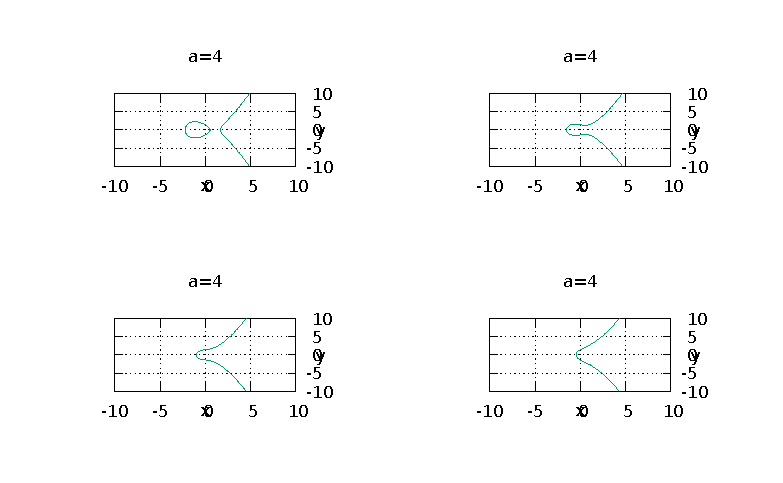
\includegraphics[angle=0]
{./add/discretmath/picelliptic.eps}
\fi
\caption{Эллиптическая кривая $y^2 = x^3 + a x + 2$ над полем
  вещественных чисел $\mathbb{R}$ при различных значениях параметра $a$}
\label{fig:add:ellipticR}
\end{figure}
